%%%%%%%%%%%%%%%%%%%%%%%%%%%%%%%%%%%%%%%%%
% SYNTHESE DE COMPUTING LINGUISTIC
% AUTEUR: DENIS GENON
%%%%%%%%%%%%%%%%%%%%%%%%%%%%%%%%%%%%%%%%%

%----------------------------------------------------------------------------------------
%	PACKAGES AND OTHER DOCUMENT CONFIGURATIONS
%----------------------------------------------------------------------------------------

\documentclass[12pt]{article} % Default font size is 12pt, it can be changed here

\usepackage{geometry} % Required to change the page size to A4
\geometry{a4paper} % Set the page size to be A4 as opposed to the default US Letter

\usepackage{graphicx} % Required for including pictures
\usepackage[USenglish]{babel} %francais, polish, spanish, ...
\usepackage[T1]{fontenc}
\usepackage[utf8x]{inputenc} %%TODO ansinew
\usepackage{lmodern} %Type1-font for non-english texts and characters
\usepackage{float} % Allows putting an [H] in \begin{figure} to specify the exact location of the figure
\usepackage{caption}
%\setlength\parindent{0pt} % Uncomment to remove all indentation from paragraphs
\usepackage{enumitem}
\setlist[enumerate]{topsep=1pt,itemsep=-1ex,partopsep=1ex,parsep=1ex}
\setlist[itemize]{topsep=1pt,itemsep=-1ex,partopsep=1ex,parsep=1ex}
\usepackage{amsmath}

\begin{document}

%----------------------------------------------------------------------------------------
%	TITLE PAGE
%----------------------------------------------------------------------------------------

\begin{titlepage}

\newcommand{\HRule}{\rule{\linewidth}{0.5mm}} % Defines a new command for the horizontal lines, change thickness here

\center % Center everything on the page

\textsc{\LARGE Université Catholique de Louvain}\\[1.5cm] % Name of your university/college
\textsc{\Large Master en Sciences de l'informatique}\\[0.5cm] % Major heading such as course name
\textsc{\large Intelligence Artificielle}\\[0.5cm] % Minor heading such as course title

\HRule \\[0.4cm]
{ \huge \bfseries LINGI2263: Computational Linguistics}\\[0.4cm] % Title of your document
\HRule \\[1.5cm]

\begin{minipage}{0.4\textwidth}
\begin{flushleft} \large
\emph{Author:}\\
Denis \textsc{Genon} % Your name
\end{flushleft}
\end{minipage}
~


%\includegraphics{Logo}\\[1cm] % Include a department/university logo - this will require the graphicx package

\vfill % Fill the rest of the page with whitespace

\end{titlepage}

%----------------------------------------------------------------------------------------
%	TABLE OF CONTENTS
%----------------------------------------------------------------------------------------

\tableofcontents % Include a table of contents

%----------------------------------------------------------------------------------------
%	SYNTHESE
%----------------------------------------------------------------------------------------
\newpage

\section{Introduction}
%!TEX root = main.tex

\subsection{What is NLP ?}

Natural language processing (NLP) is a field of computer science, artificial intelligence, and computational linguistics concerned with the interactions between computers and human (natural) languages. There is differents applications:
\begin{itemize}
	\item Communicating agent;
	\item Translator;
	\item Information extraction;
	\item Inference of knowlegde;
	\item \dots
\end{itemize}

\subsection{Three approches to NLP}

\begin{enumerate}
	\item \textbf{Symbolic}: Use of language ressources (dictionnaries, grammars, thesaurus, \dots);
	\item \textbf{Statistical}:  Use of empirical techniques to learn from text and construct language models;
	\item \textbf{Hybrid}: Combining language ressources and statistical algorithms.
\end{enumerate}

\subsection{Basic linguistics concepts}

\subsubsection{Language vs. languages}

\begin{itemize}
	\item \textbf{A language}: A system of spoken/written communication used by a particular country, people, \dots typically consisting of words used within a regular grammatical and syntactic structure;
	\item \textbf{The language}: Power or faculty of speech.
\end{itemize}


\subsubsection{Competence vs. performance}

\begin{itemize}
	\item \textbf{Competence}: knowledge of a language;
	\item \textbf{Performance}: Use of language in concrete situation.
\end{itemize}

\subsubsection{Nature of the linguistic sign}

\textit{Words} are \textit{linguistic signs}. They convey some idea.

\noindent
\begin{minipage}{.5\textwidth}
	\begin{itemize}
		\item \textbf{Signifier}: The psychic imprint of the sound (not the sound);
		\item \textbf{Signified}: The concept associated to the signifier;
		\item \textbf{Referent}: Actual \textit{object} in the real world.
	\end{itemize}
\end{minipage}%
\begin{minipage}{.5\textwidth}
	\centering
	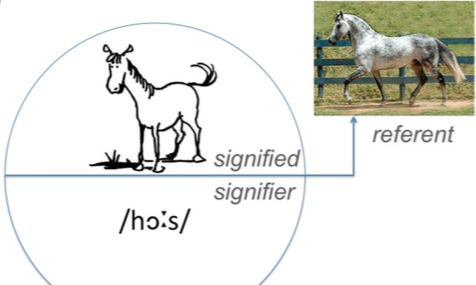
\includegraphics[scale=0.4]{images/01_nature.png}
 	\captionof{figure}{Nature of linguistic sign.}
\end{minipage}

\vspace{10px}

The linguistic sign has the three following characteritics:

\begin{itemize}
	\item \textbf{Arbitrary}: The relationship between the signifier and the signified is not motivated;
	\item \textbf{Conventional}: The link is based on social conventions;
	\item \textbf{Differential}: Signs are part of a system.
\end{itemize}


\subsubsection{Double articulation of the language}

A double articulation caracterize human languages.

\begin{itemize}
	\item At first level, \textbf{morpheme} (or moneme) are the smallest meaningful units. A \textbf{morph} is a concrete realisation of a morpheme. For example, the morphene \textit{take} has two realizations: \textit{take, took}. The variants of a same morpheme are called \textbf{allomorphs};
	\item At a second level, \textbf{phonemes} are the smallest distinctive units. A \textbf{phone} is a realisation of a phoneme. Variants of a given phoneme are called \textbf{allophone} (livre and ville).
\end{itemize}

\subsubsection{Two axes: syntagmatic vs. paradigmatic}

\noindent
\begin{minipage}{.4\textwidth}
	Morphemes can be replaced by others on the \textbf{paradigmatic} axis (vertical) or they can appear in a different environement, combined with other morphemes on the \textbf{syntagmatic} axis (horizontal).
\end{minipage}%
\begin{minipage}{.6\textwidth}
	\centering
	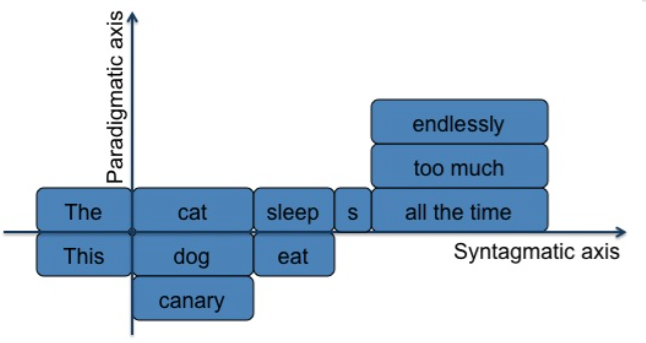
\includegraphics[scale=0.4]{images/02_axis.png}
 	\captionof{figure}{The two axes.}
\end{minipage}

\subsubsection{Other general linguistic considerations}

\begin{itemize}
	\item \textbf{Creativity}: Finite number of signs permit to elaborate an infinite number of utterences;
	\item \textbf{Evolutivity}: Languages change over the time;
	\item \textbf{Complexity}: Languages are of equal complexity.
\end{itemize}

\subsection{Levels of a linguistic analysis}

\begin{figure}[htp]
	\centering
	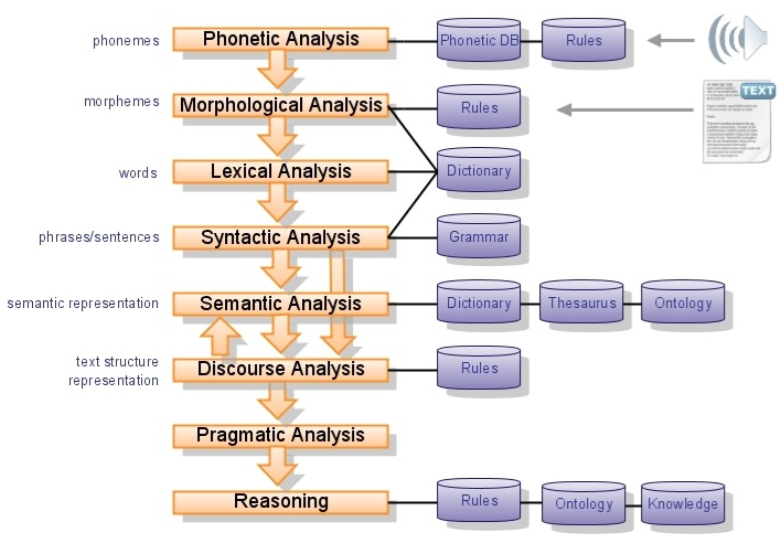
\includegraphics[scale=0.4]{images/03_levels.png}
 	\caption{Different levels of linguistic analysis.}
\end{figure}

\subsubsection{Phonology}

It is the systematic study of the sounds used in language, and their composition into syllables, words, phrases. Computational phonology is the application of formal and computational techniques to the representation and processing of phonological information.

\vspace{10px}
There is several applications:
\begin{itemize}
	\item Speech recognition;
	\item Speech synthesis;
	\item Phonetic algorithms;
	\item \dots
\end{itemize}

\subsubsection{Morphology}

The notion of word is ambiguous:
\begin{itemize}
	\item \textbf{Tokens}: Number of words; \textbf{Types}: Number of unique words.
	\item \textbf{Phonemic} words: \textit{[hai]}; \textbf{Graphemic} words: \textit{high}.
	\item \textbf{Mono-lexical} unit: \textit{feuille}; \textbf{Polylexical} unit: \textit{arc-en-ciel}.
	\item \textbf{Function} word: \textit{to, from}; \textbf{Full} word: \textit{home, sea}.
\end{itemize}

\vspace{10px}

There is too abstract notions behind words:
\begin{itemize}
	\item \textbf{Lemma}: Is the cannonical form of a word (entry of a dictionary, infinitive form or masculine form);
	\item \textbf{Part of Speech}: Are grammatical categories indentifying the nature and/or syntactic function of a word.
\end{itemize}

\vspace{10px}

Morphene are abstract entities expressing semantic concepts or grammatical features.

\begin{figure}[htp]
	\centering
	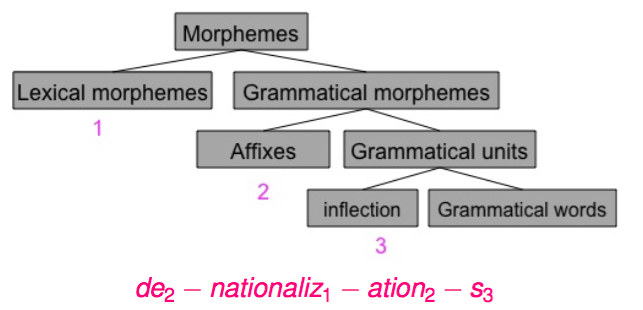
\includegraphics[scale=0.4]{images/04_tree.png}
 	\caption{Grammatical and Lexical morphology.}
\end{figure}

There is several ways to create new words:

\begin{itemize}
	\item \textbf{Inflection}: Grammatical adaptation of a word in a particular syntactic contexts (grammatical morphology);
	\item \textbf{Derivation}: Creation of a new word by adding a bound morpheme (affix) to a derivational base (lexical morphology);
	\item \textbf{Composition}: joining of two or more base forms: hot pepper, cool-headed, online, \dots
\end{itemize}

\vspace{10px}


There are three main aspects linked to morphological analysis:

\begin{itemize}
	\item \textbf{Lemmatization \& Stemming}: The goal is to reduce inflectional forms and sometimes derivationally related forms of a word to a common base form.
	\begin{itemize}
		\item \textbf{Lemmatization}: Based on morphological dictionnaries and analyzers. \textbf{Morphological analyser}  are able to analyze new words using a base dictionary (words and affixes) and morphological rules (add/remove affixes). \textbf{Morphological dictionaries} contain forms, lemma, morphological information, \dots.
		\item \textbf{Stemming}: Based on predefined rules.\\
		Algorithm of Porter: 
		\begin{enumerate}
			\item Check if word respect some form;
			\begin{figure}[htp]
				\centering
				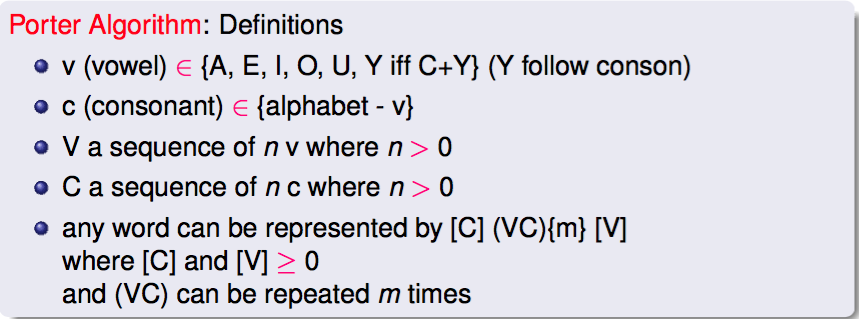
\includegraphics[scale=0.4]{images/05_form.png}
			\end{figure}
			\item If word respect some form, apply 5 runs of somes rules.
			\begin{figure}[htp]
				\centering
				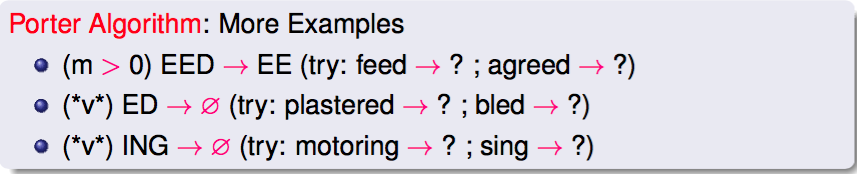
\includegraphics[scale=0.4]{images/06_rule.png}
			\end{figure}
		\end{enumerate}
		There is two typical problems: \textbf{Under-stemming} error (algo failed to group two words sharing conceptual meaning: divide and division does not give the same result); \textbf{Over-stemming} error (algo grouped words having no shared conceptual meaning: wand and to wander).
	\end{itemize}
	\item \textbf{POS Tagging}: labeling word with POS (rules vs probabilities);
	\item \textbf{Disambiguation}: Clarify the nature or function of a word in a sentence.
\end{itemize}


\subsubsection{From lexis to syntax}

Lexicalization is the process of adding words, set phrases, or word patterns to a language. This step is complicated for \textbf{compound words} and \textbf{frozen expressions}.

\section{Corpus}
%!TEX root = main.tex

\subsection{What is a corpus ?}

A large body of linguistic evidence typically composed of attested language use.

There is several desired characteristics of a corpus:
\begin{itemize}
	\item Machine readable;
	\item Sampled (aiming at balance and representativeness);
	\item Well-organized and formatted;
	\item Big.
\end{itemize}

\subsubsection{Whats is a corpus for ?}

\begin{itemize}
	\item For linguists:
	\begin{itemize}
		\item Empirical approach (based on facts)
		\item Chomsky does not like it because it captures bits of performance but not competence. 
	\end{itemize}
	\item In NLP: the raw fuel of NLP.
\end{itemize}

\subsubsection{Typology}

There is two category of corpus: \textbf{monolingual} and \textbf{multilingual}. The first one has three types:
\begin{itemize}
	\item \textbf{Reference corpus}: large, balanced and \textit{representative}, it is designed to provide comprehensive information about a language;
	\item \textbf{Specialized corpus}: corpus designed to cover one particular aspect of the language;
	\item \textbf{Static} vs. \textbf{Monitor corpus}: Static corpus does not evolve.
\end{itemize}

The second one (\textbf{multilingual}) has two types:
\begin{itemize}
	\item \textbf{Comparable corpora}: several corpora of various languages collected using the same sampling method and similar balance in order to permit comparisons between corpora;
	\item \textbf{Parallel corpora}: gather a corpus in one language and the translation of this corpus in one or more orther languages.
\end{itemize}

\subsubsection{Collection}

\textbf{Oral corpora} are collected from recordings of interview, conferences, radio or TV programs, \dots \textbf{Written corpora} are collected from digitalization of analogical sources, digital sources, web, \dots

\subsection{Corpus Annotation}

The aim of corpus annotation is to make explicit some linguistic infor- mation that is part of the text. This is done by adding metadata to the text. Automatic or manual.

There is 6 levels of annotations:
\begin{itemize}
	\item morpho-syntactic annotation;
	\item lemmatization;
	\item syntactic annotation (treebanks);
	\item semantic annotation (entities, word meaning, predicates, etc.);
	\item discourse annotation (ie: anaphora);
	\item phonetic transcription.
\end{itemize}

\begin{figure}[htp]
	\centering
	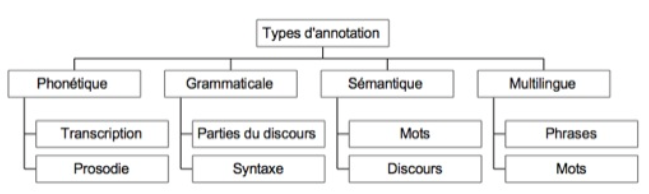
\includegraphics[scale=0.6]{images/07_levels.png}
 	\caption{Levels of annotation.}
\end{figure}

There is some standards for annotation: the goal is to ensure corpora \textbf{reusability} and software \textbf{interoperability}.

\subsection{Corpus Processing}

Here is the typical steps of corpus processing:
\begin{itemize}
	\item \textbf{Text formatting and normalization}
	\item \textbf{Tokenization}: Sevral ways to do it. Type/Token Ratio.
	\item \textbf{Lexical analysis}
	\begin{itemize}
		\item \textbf{Morphological analysis}: Based on dictionary and morphological rules. On the fly and can process new words. If only dictionary based, it is quick but limited on the dictionary coverage.
		\item \textbf{POS tagging}: Remove ambiguity (walk: noun or verb ?)
		\item \textbf{Lemmatization}
	\end{itemize}
	\item \textbf{Entitites recognition}
	\item \textbf{Syntactic analysis}
	\item \dots
\end{itemize}


\section{Ngrams}
%!TEX root = main.tex
\subsection{Introduction}
In N-Grams, each word occurence is considered as a random event.
\subsubsection{Zipf's law}

The count histogram follow the Zipf's law: $y = bx^{-a}$.

\begin{figure}[htp]
	\centering
	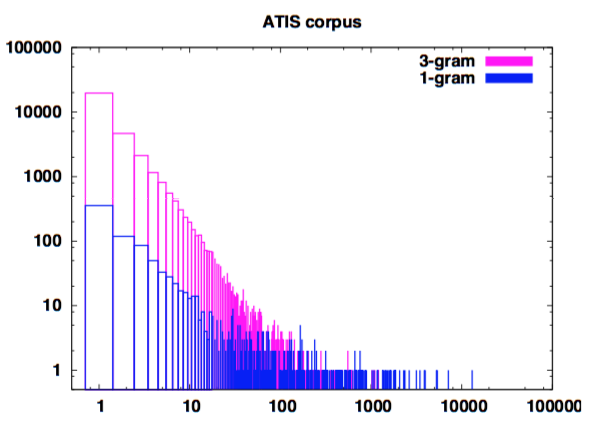
\includegraphics[scale=0.4]{images/08_zipf.png}
 	\caption{Zipf's law.}
\end{figure}

\subsubsection{N-Gram probability}

\begin{figure}[htp]
	\centering
	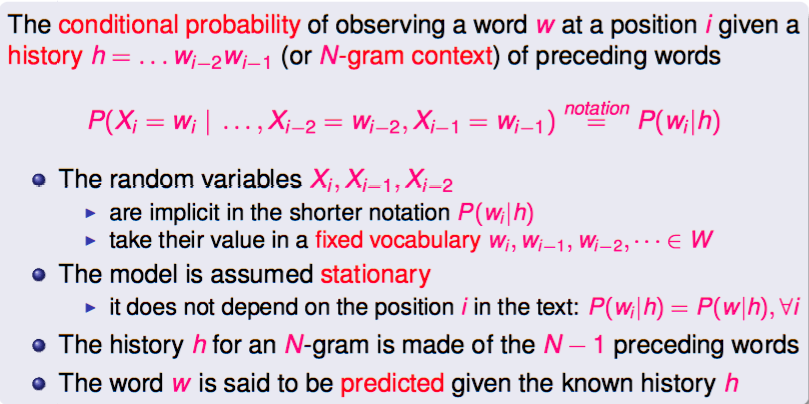
\includegraphics[scale=0.4]{images/09_proba.png}
 	\caption{N-Gram probability.}
\end{figure}

We can then compute a sentence probability if we use the chain rule and the N-Gram assumption.

\begin{figure}[htp]
	\centering
	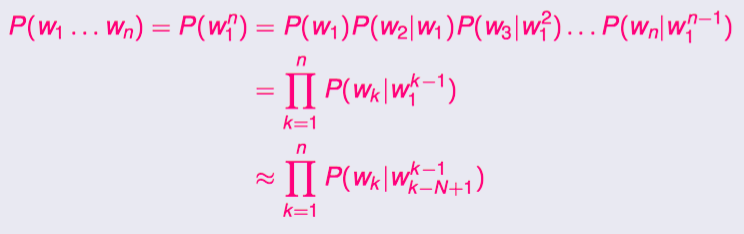
\includegraphics[scale=0.4]{images/10_sentence.png}
 	\caption{Sentence probability.}
\end{figure}

For example (3-gram): P(The rain in Spain) $\approx$ P(The) $*$ P(rain | The) $*$ P(in | The rain) $*$ P(Spain | rain in).

\subsubsection{Consistency property}

Must be verified for all models.

\begin{figure}[htp]
	\centering
	
\includegraphics[scale=0.5]{images/11_consistency.png}
 	\caption{Consistency property.}
\end{figure}
\subsection{N-Gram estimation}

\subsubsection{Maximum Likelihood estimation}

\begin{figure}[htp]
	\centering
	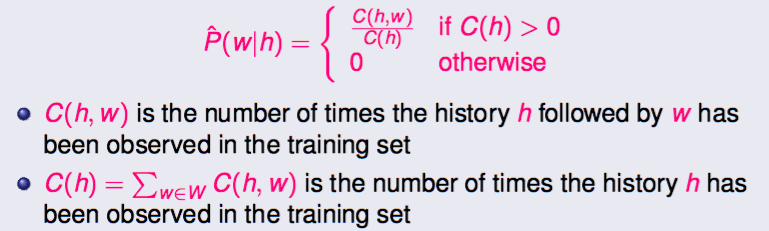
\includegraphics[scale=0.5]{images/12_likelihood.png}
 	\caption{Maximum likelihood estimation.}
\end{figure}

For unigram, $\hat{P}(w) = \frac{C(w)}{N}$ where $N$ is the size of the corpus.

\subsection{Smoothing}

Smoothing is necessary because MLE assign a zero probability to any unseen events in the training set. Many possible events are assigned a zero probability and the probability of observed events is overestimated. Smoothing techniques must respect the consistency property.

\subsubsection{Bayesian estimation}

The goal of bayesian estimation (or additive smoothing) is to add a pseudo count to avoid having probabilities of 0 for unseen events in the traning set.

\begin{figure}[htp]
	\centering
	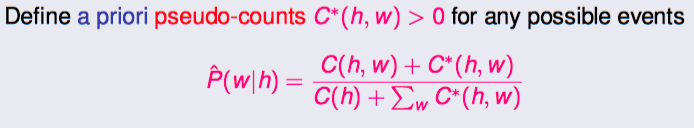
\includegraphics[scale=0.5]{images/13_bayesian.png}
 	\caption{Bayesian estimation.}
\end{figure}

The \textbf{prior probability} of the event $(h,w)$ is defined as $\frac{C^*(h,w)}{\sum_w C^*(h,w)}$. $\hat{P}(w|h)$ can be interpreted as a \textbf{posterior estimate}.

A particular form of the bayesian smoothing is the \textbf{Laplace} smoothing (or add one method).

\begin{figure}[htp]
	\centering
	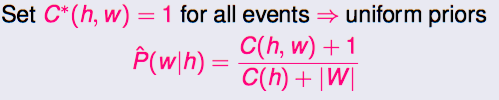
\includegraphics[scale=0.5]{images/14_add_one.png}
 	\caption{Add one method.}
\end{figure}

In general add-one smoothing is a poor method of smoothing because too much probability mass is moved to all the zeros.


\subsubsection{Linear estimation}

The goal is to build different estimators for several model orders. The differents estimators vary by history and are combined linearly.

\begin{figure}[htp]
	\centering
	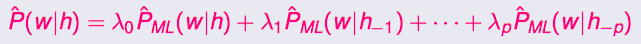
\includegraphics[scale=0.5]{images/15_linear.png}
 	\caption{Linear interpolation. $h_{-1}$: $h$ without the front word.}
\end{figure}

We need then to estimate the weights of the model: \textbf{Expectation-Maximization estimation}. The model before is a special case of the \textbf{mixture model}.

\begin{figure}[H]
	\centering
	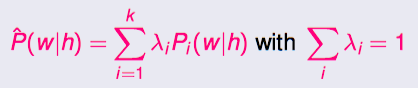
\includegraphics[scale=0.5]{images/16_mixture.png}
 	\caption{Mixture model.}
\end{figure}

We can estimate the $\lambda$'s with this algorithm:

\begin{figure}[htp]
	\centering
	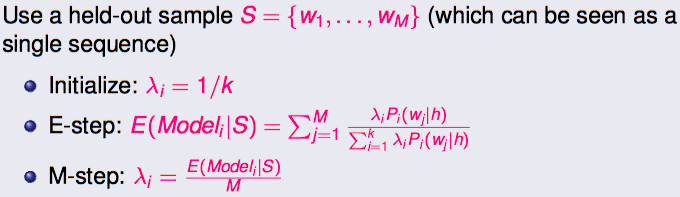
\includegraphics[scale=0.5]{images/17_em.png}
 	\caption{Expectation-Maximization algorithm.}
\end{figure}

\subsubsection{Backoff smoothing}

Idea: if we have no examples for a particular trigram, we can estimate its probability by using his bigram probability (backoff). 

\begin{figure}[H]
	\centering
	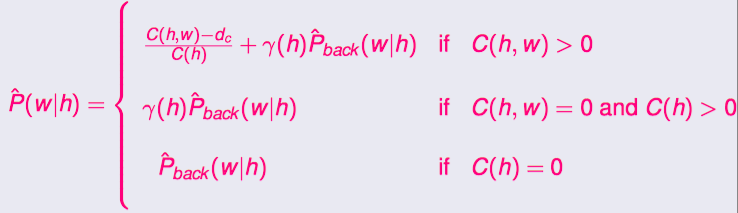
\includegraphics[scale=0.5]{images/18_backoff.png}
 	\caption{Backoff smoothing. $\hat{P}_{back}(w|h) = \hat{P}(w|h_{-1})$.}
\end{figure}

$d_c$ are the \textbf{discounting coefficients}, and $\gamma(h) = \sum_{w:C(h,w)>0} \frac{d_c}{C(h)}$.

\begin{figure}[htp]
	\centering
	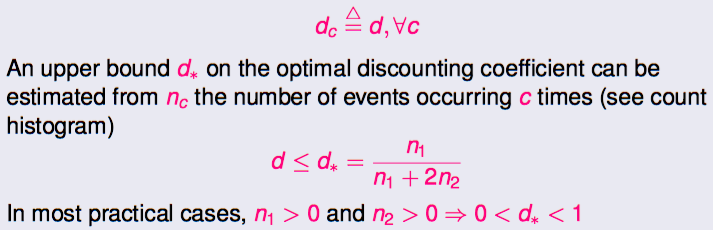
\includegraphics[scale=0.5]{images/19_discounting.png}
 	\caption{Absolute discounting.}
\end{figure}

\subsection{Performance assessment}

To test the smoothing, we can do \textbf{data splitting}:

\begin{itemize}
	\item \textbf{Basic protocol}: split data to into training (90\%, estimate the model) and test (10\%, evalute the quality of the model) files.
	\item \textbf{Refinement 1}:
	\begin{itemize}
		\item Split training set into 90\% of actual training and 10\% of held-out set (used to tune \textit{meta-parameters}: pseudo counts or $\lambda$'s and select an optimal model order)
		\item Re-train on the whole training set with any meta-parameter being fixed.
	\end{itemize}
	\item \textbf{Refinement 2}: Repeat the above using 10-fold cross validation. 
\end{itemize}

We can compute the \textbf{perplexity} too. The perplexity is a measure of quality of an iterated Shannon game.

\begin{figure}[H]
	\centering
	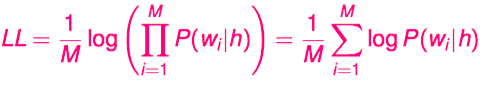
\includegraphics[scale=0.5]{images/20_log.png}
 	\caption{Per-symbol log likelihood.}
\end{figure}

\begin{figure}[H]
	\centering
	
\includegraphics[scale=0.6]{images/21_perplexity.png}
 	\caption{Test set perplexity. If random (uniform) over W, $PP = |W|$. Lower the better.}
\end{figure}

If there is a word we have never see, even with a consistent and smoothed model, $P(w_{new}|h) = 0$, $PP = +\infty$. The astuce is to define a \textit{UNK} word as part of the vocabulary and relies on smoothing. 

\section{HMMs}
%!TEX root = main.tex

A motivating example is the POS tagging. The goal is to assign a POS tag to each word of a sentence. This tagging is ambiguous, so we will choose a tag according to the context of the word. Words are observed and tags are hidden. We will use a finite state model where tags are states and tagging a sentence reduces to find the most likely state sequence.

\subsection{Markov Chains}

\begin{figure}[htp]
	\centering
	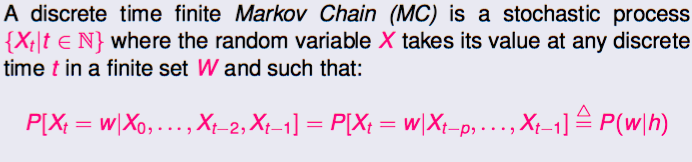
\includegraphics[scale=0.5]{images/22_chains.png}
 	\caption{A Markov chain of order p is a N-Gram model with $N = p+1$. }
\end{figure}

\begin{figure}[htp]
	\centering
	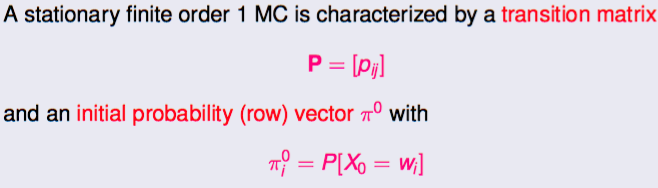
\includegraphics[scale=0.6]{images/23_prob.png}
 	\caption{Transition and initial probabilities.}
\end{figure}


\begin{figure}
\centering
\begin{minipage}{.5\textwidth}
  \centering
  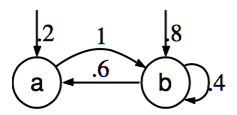
\includegraphics[scale=0.6]{images/24_ex1.png}
\end{minipage}%
\begin{minipage}{.5\textwidth}
  \centering
  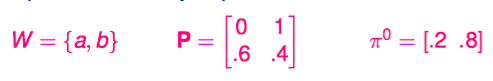
\includegraphics[scale=0.5]{images/25_ex2.png}
\end{minipage}
\end{figure}

The maximal number of states $|W|^p$ grows exponentially with $p$.

\begin{figure}[htp]
	\centering
	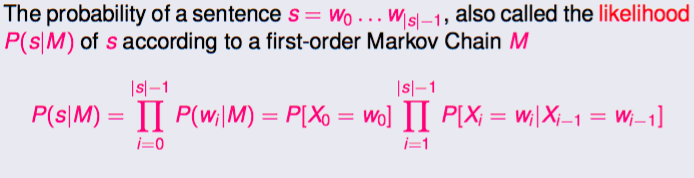
\includegraphics[scale=0.5]{images/26_sentence.png}
 	\caption{A sentence probability for a Markov Chain.}
\end{figure}

\subsection{Hidden Markov Models}

\begin{figure}[H]
	\centering
	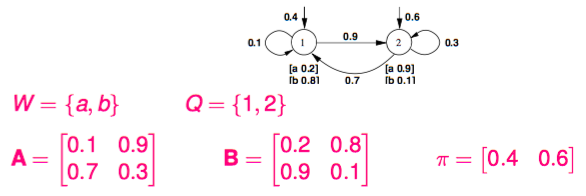
\includegraphics[scale=0.5]{images/27_ex1.png}
\end{figure}

\begin{figure}[H]
	\centering
	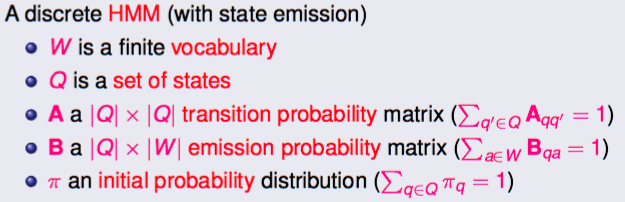
\includegraphics[scale=0.5]{images/28_ex2.png}
\end{figure}

\subsubsection{Path likelihood}
\begin{figure}[htp]
	\centering
	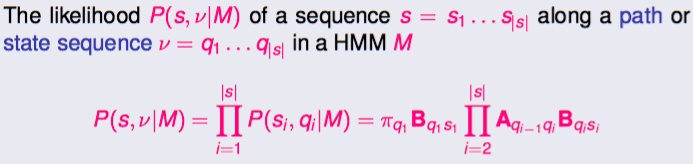
\includegraphics[scale=0.6]{images/29_path.png}
 	\caption{Path likelihood.}
\end{figure}

\subsubsection{Sequence likelihood}
Complicated because $O(|Q|^{|S|})$ possible state sequences ($|Q|$ is number of states and $|S|$ is sequence length).


\subsection{Most likely state sequence}

\begin{figure}[htp]
	\centering
	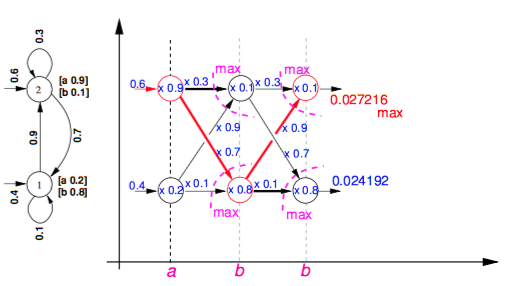
\includegraphics[scale=0.6]{images/30_viterbi.png}
 	\caption{Example.}
\end{figure}

\begin{figure}[htp]
	\centering
	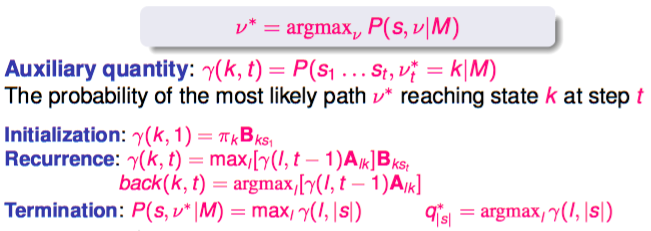
\includegraphics[scale=0.6]{images/31_viterbi.png}
 	\caption{Viterbi decoding (recurrence) Algorithm.}
\end{figure}

\begin{itemize}
	\item $P(s, v^*)$ gives the probability of the optimal path $v^*$;
	\item Computation are done with log (because too small values);
	\item Complexity: $\Theta(m|s|)$;
	\item Path $v^*$ is an alignement between states and words;
	\item $v^*$ can be recovered with the backpointers.
\end{itemize}

\newpage

\subsection{Sequence likelihood}

\begin{figure}[htp]
	\centering
	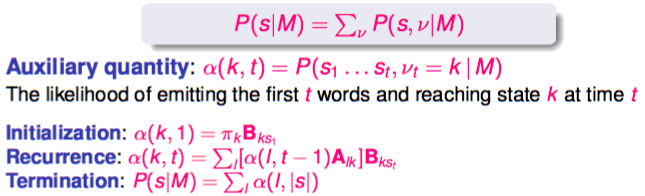
\includegraphics[scale=0.6]{images/32_forward.png}
 	\caption{Forward recurrence, same complexity as viterbi recurrence.}
\end{figure}

\subsection{The learning problem}

Given an HMM structure and several sentences, you must estimate $A$, $B$, $\pi$.

\subsubsection{Supervised}

The learning sentences are annoted with their respective states.

\begin{figure}[htp]
	\centering
	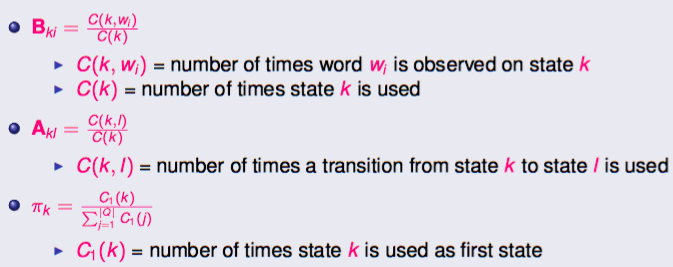
\includegraphics[scale=0.6]{images/33_supervised.png}
 	\caption{Supervised learning.}
\end{figure}


\subsubsection{Unsupervised}

The sentences are not annoted. There is two algorithm. The first one is \textbf{Viterbi training}.

\begin{figure}[htp]
	\centering
	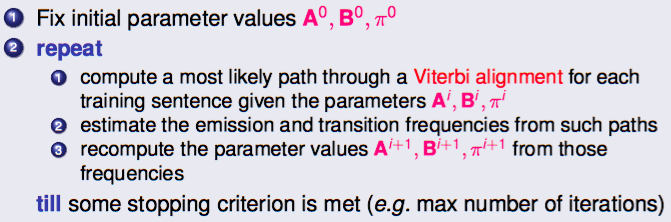
\includegraphics[scale=0.6]{images/34_viterbi.png}
 	\caption{Viterbi learning.}
\end{figure}

The second is \textbf{Forward-Backward} or \textbf{Braaum-Welch} algorithm. Viterbi training is an approximation as it considers that each training sentence is generated along a single path. A more accurate estimation is obtained if one considers all possible paths to generate each sentence.

\begin{itemize}
	\item actual frequencies ($C(k, w_i)$, $C(k)$, $C(k, l)$, \dots ), are replaced by expected frequencies;
	\item   special case of expectation-maximization (EM) procedure
\end{itemize}

Viterbi and Baum-Welch training are both sensitive to parameter initialization.





\section{POStagging}
%!TEX root = main.tex

\subsection{Rule-based approach}

Use a large dictionary to assign each word a set of possible tags. Apply a large list of disambiguation rules to restrict each set to a single tag for each word. The constraints are used in a negative way, to eliminate the tags that are inconsistent with the context.

\begin{figure}[htp]
	\centering
	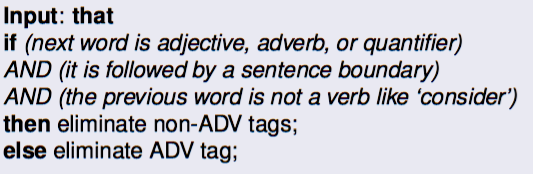
\includegraphics[scale=0.4]{images/35_rules.png}
 	\caption{Example of rules.}
\end{figure}

There are some limitations:
\begin{itemize}
	\item Specific to a given language;
	\item Linguistics ressource need to be updated. 
\end{itemize}

\subsection{Probabilistic approach}

See previous chapter.

\subsection{Transformation-based tagging}

\begin{figure}[htp]
	\centering
	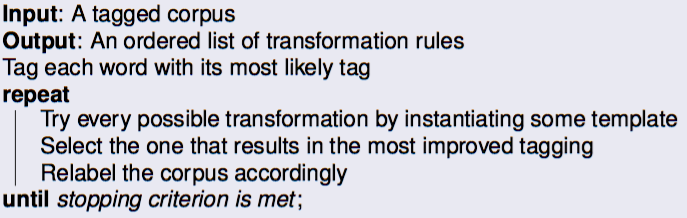
\includegraphics[scale=0.4]{images/36_brill.png}
 	\caption{Brill tagger.}
\end{figure}
 The algorithm need transformations templates (Change tag from \textbf{a} to \textbf{b} when word before is tagged \textbf{z}, \dots) and a tagged corpus. A stopping criterion could be: insufficient improvement over the previous pass. To know if the transformation give a better tagging, the algorithm need a tagged corpus. The output of the TBL process is an ordered list of transformations; these then constitute a tagging procedure that can be applied to a new corpus. 

  \subsubsection{Pros}
  \begin{itemize}
  	\item Transformations rules can be interpreted linguistically;
  	\item Learning those rules makes it possible to adapt the tagger to several languages.
  \end{itemize}
  \subsubsection{Limitations}
  \begin{itemize}
  	\item A transformation rule can be learned only if it is an instance of an abstract transformation template;
  	\item Supervised only, need a tagged corpus;
  	\item Computational complexity of learning is an issue.
  \end{itemize}

\subsection{HMM POS tagging}

\subsubsection{Supervised learning}

\begin{figure}[H]
	\centering
	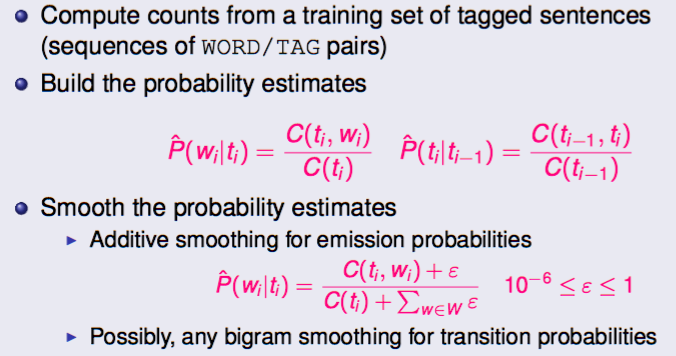
\includegraphics[scale=0.5]{images/38_supervised.png}
 	\caption{HMM tagging = Viterbi decoding.}
\end{figure}

\paragraph{Pro}

We can interpret the states as true POS tag and there is no need to discover the meaning of the states after learning.

\paragraph{Limitations}

A tagged corpus is required.

\subsubsection{Unsupervised learning}
\begin{figure}[H]
	\centering
	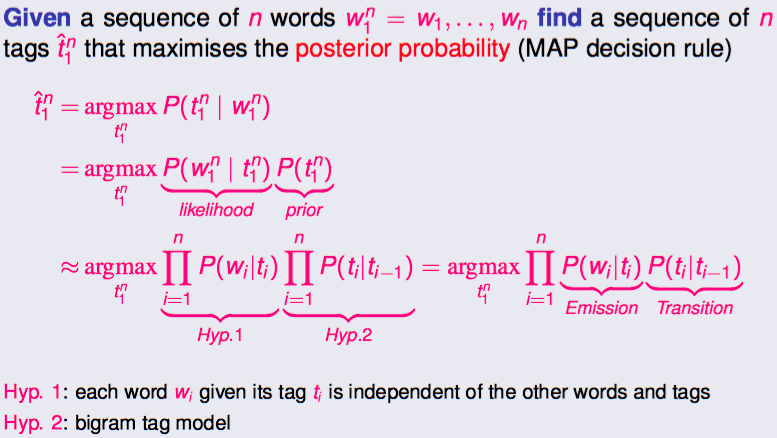
\includegraphics[scale=0.45]{images/37_viterbi.png}
 	\caption{HMM tagging = Viterbi decoding.}
\end{figure}
\paragraph{Pro}

Fully automatic. Define a HMM structure with one state per tag in a tagset and learn the HMM parameters $P(w_i|t_i)$ and $P(t_i|t_{i−1})$ using Viterbi training or Baum-Welch on a text corpus (not tagged!).

\paragraph{Limitations}

Viterbi training and Baum-Welch are sensitive to the initialization. The states are not necessarily associated with relevant tag set, some linguistically informed post-processing needs to be done if one wants to map states to actual tags, whenever possible.

\subsubsection{Notes}

A \textbf{out-of-vocabulary} word in the test set is assigned as a zero probability, there is no Viterbi path. The usual solution is to replace any word occuring only once in the training set with the marker \textit{UNK}. We then need to reduce the observed vocabulary and add \textit{UNK} to it and smooth the emission probability.\\

It is possible to extend HMM to tag trigrams.

\begin{figure}[H]
	\centering
	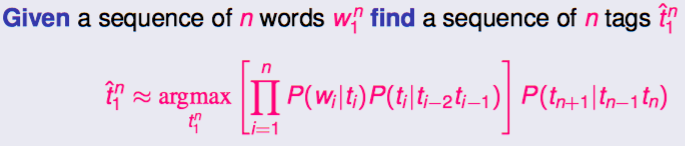
\includegraphics[scale=0.5]{images/39_trigrams.png}
 	\caption{Need to apply n-gram smoothing techniques.}
\end{figure}

\subsection{Evaluation}

\begin{figure}[H]
\centering
\begin{minipage}{.5\textwidth}
  \centering
  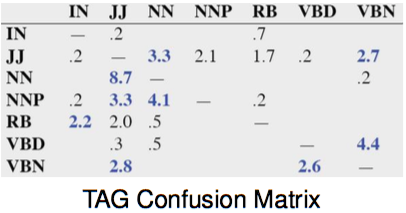
\includegraphics[scale=0.5]{images/40_matrix.png}
\end{minipage}%
\begin{minipage}{.5\textwidth}
  \centering
  \begin{itemize}
  	\item Row is an actual tag;
  	\item Column is predicted tag;
  	\item Entry is error percentage.
  \end{itemize}
\end{minipage}
\end{figure}

There is the formula to assess the perfomance of the tagging.

\begin{itemize}
	\item \textbf{Average error rate per TAG} = $\frac{1}{\# of rows}*\sum_i (\text{total of row i})$;
	\item \textbf{Tagging error rate} = $\frac{\sum_i f(i)*(\text{total of row i})}{\sum_i f(i)}$;
	\item \textbf{Tagging accuracy} = $100\% - \text{Tagging error rate}$.
\end{itemize}

\section{Formal Grammar}
%!TEX root = main.tex

The \textbf{syntax} correspond to an arrangement to form correct sentences. A \textbf{formal grammar} is the set of rules which define the syntax. The \textbf{syntactic analysis} is the application of formal rules to filter grammatical and ungrammatical sentences. There is three fundamental concepts in formal grammar.

\begin{itemize}
	\item \textbf{Constituency}: a group of words may behave as a single unit. For example, nominal sentences. There is two clues of words that are grouped togheter: the first one is the context (before a verb for example) and the second is that we can move the group of word in different places of the sentence (preposed/postposed constructions);
	\item \textbf{Grammatical relations}: formalization of ideas from traditional grammar (Subject/Object);
	\item \textbf{Subcategorization and dependency relations}: Some types of relations between word and phrases (for example transitive verbs like \textit{find}).
\end{itemize}

\subsection{Context Free Grammar}

A CFG consists of a set of rules and a lexicon of words and symbols.
\begin{itemize}
	\item $N$ a set of non-termina symbols;
	\item $\sum$ a set of terminal symbols;
	\item $R$ a set of rules of the form $A \rightarrow \beta$;
	\begin{itemize}
		\item $A$ is non-terminal;
		\item $\beta$ is a string of symbols: $(N \cup \sum)^*$.
	\end{itemize}
	\item $S$ a start symbol.
\end{itemize}

A CFG define a formal language. The term generative grammar underlines the fact that in this approach a language is defined by a set of possible sentences generated by the grammar.

\subsection{Some grammar rules and syntactic structures}

\subsubsection{Agreement problem}

To handle the particular cases (for example a verb which take \textit{s} at the third singular form), we need to add rules on the grammar. The consequence is a increase of the size of the grammar. A solution is to use a constraint-based formalism to take into accont fine-grained information about number and person agreement, subcategorization and even semantic categories.

\begin{figure}[htp]
	\centering
	
\includegraphics[scale=0.4]{images/41_matrix.png}
 	\caption{Feature structure.}
\end{figure}

\subsubsection{Subcategorization}

All verbs are not compatible with all kind of constituents. The solution is to have different catagories of words (for example, transitive verb and instransitive verb).

\subsubsection{Treebank}

\begin{figure}[htp]
	\centering
	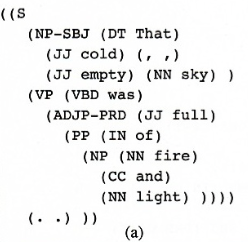
\includegraphics[scale=0.4]{images/42_treebank.png}
 	\caption{Brown treebank.}
\end{figure}

\subsection{Dependency Grammars}

In dependency grammars, constituents and phrase structure rules do not play any fundamental role. Instead, the syntactic structure of a sentence is described purely in terms of words and binary semantic or syntactic relations between these words (called lexical dependencies). Dependency grammars use dependency relationships between lexicon elements. The nature of the relationship can be morphologic, syntaxic or semantic. The main advantage is to handle languages with free word order (Czech, Latin).

\section{Syntactic Parsing}
%!TEX root = main.tex

\subsection{Introduction}

\textbf{Problem}: Given a formal grammar G (CFG) and a sentence s, build a parse tree of s according to G. There may be no solution or many solutions (ambiguity). Context-free means that any rules used to replace the left hand side can be used anywhere in a parse tree.

\textbf{Parsing} is the search among all possible parse trees that can be generated from S for the one generating the observed sentence s. The search space can be explored \textbf{bottom-up} or \textbf{top-down}.
\\ 
\noindent
\begin{minipage}{.5\textwidth}
	\centering
	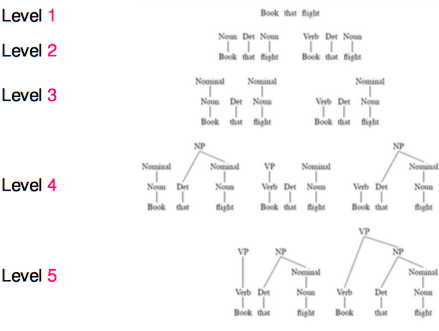
\includegraphics[scale=0.4]{images/43_bottom-up.png}
 	\captionof{figure}{Bottom-up. Never wastes time exploring tree that cannot result is an S.}
\end{minipage}%
\begin{minipage}{.5\textwidth}
	\centering
	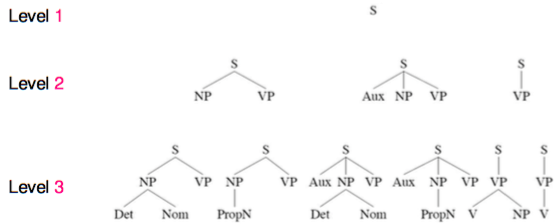
\includegraphics[scale=0.4]{images/44_top-down.png}
 	\captionof{figure}{Top-down. Never wastes time on trees that are not consistent with the input.}
\end{minipage}

Due to ambiguity, in the worst case, the number of parse trees is exponential to the sentence length.

\subsection{CYK Algorithm}

Before using the algorithm, we need to change the grammar in Chomsky Normal Form.

\begin{figure}[htp]
	\centering
	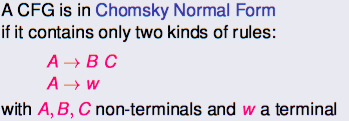
\includegraphics[scale=0.5]{images/45_chomsky.png}
 	\caption{CNF.}
\end{figure}

\begin{figure}[htp]
	\centering
	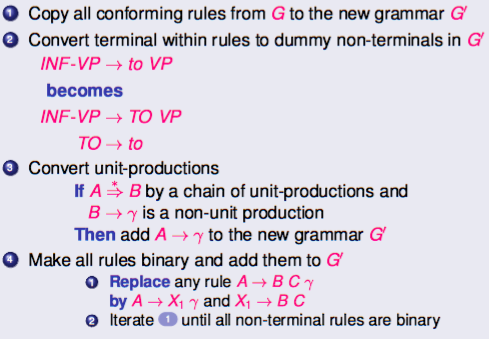
\includegraphics[scale=0.5]{images/46_conversion.png}
 	\caption{Conversion algorithm.}
\end{figure}

\begin{figure}[H]
	\centering
	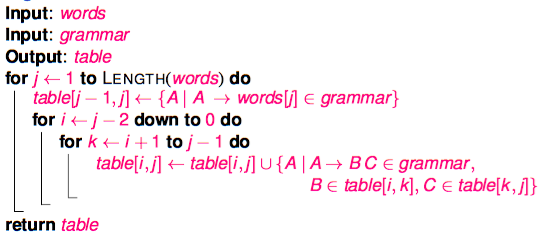
\includegraphics[scale=0.6]{images/47_cyk.png}
 	\caption{CYK algorithm. The sentence is accepted if S in $table[0,N]$. Backpointers. Bottum-up. $O(n^3)$.}
\end{figure}

\noindent
\begin{minipage}{.5\textwidth}
	\centering
	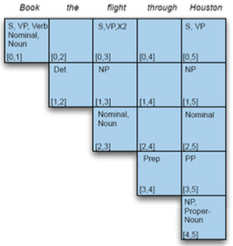
\includegraphics[scale=0.6]{images/48_table.png}
 	\captionof{figure}{Example.}
\end{minipage}%
\begin{minipage}{.5\textwidth}
	\centering
	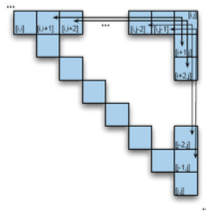
\includegraphics[scale=0.6]{images/49_order.png}
 	\captionof{figure}{Order.}
\end{minipage}


\subsection{Probabilistic CFG and probabilistic parsing}

\textbf{Problem}: Given a PCFG G and a sentence S, compute a most likely parse tree.

\begin{figure}[htp]
	\centering
	\includegraphics[scale=0.6]{images/54_prob.png}
 	\caption{Disambiguation rule.}
\end{figure}

Solve the exponential blow-up issue by computing most likely parse tree.

\begin{figure}[H]
	\centering
	\includegraphics[scale=0.6]{images/55_prob.png}
 	\caption{Probabilistic CYK.}
\end{figure}

\subsubsection{Learning rule probabilities from a Treebank}

\begin{figure}[H]
	\centering
	\includegraphics[scale=0.5]{images/56_learning.png}
 	\caption{Rule probability estimate. Smoothing may be used. Unsupervised learning possible: Inside-Outside algorithm.}
\end{figure}

\subsection{Earley Algorithm}

\begin{figure}[htp]
	\centering
	\includegraphics[scale=0.6]{images/50_earley.png}
 	\caption{Earley algorithm. Top-down. No need for CNF. A state $S \rightarrow \alpha \bullet , [0,N]$ in $chart[N]$ denotes a successful parse. $O(n^3)$. }
\end{figure}

\begin{figure}[htp]
	\centering
	\includegraphics[scale=0.5]{images/51_predictor.png}
 	\caption{Predictor.}
\end{figure}

\begin{figure}[htp]
	\centering
	\includegraphics[scale=0.5]{images/52_scanner.png}
 	\caption{Scanner.}
\end{figure}

\begin{figure}[htp]
	\centering
	\includegraphics[scale=0.5]{images/53_completer.png}
 	\caption{Completer.}
\end{figure}

\subsection{Partial parsing}

A style of partial parsing is \textbf{chunking}: a simple bracketing without hierarchical structure. 

\subsubsection{Algorithms}

\begin{itemize}
	\item HMMs;
	\item Local classifier from selected features;
	\item Iterated chunking based on a hierarchy of chunk tag offers an approximation to full parsing.
\end{itemize}

\subsubsection{Chunking system evaluation}

\begin{figure}[htp]
	\centering
	\includegraphics[scale=0.6]{images/57_eval.png}
 	\caption{Evaluation. State of art is 92\% $F_1$.}
\end{figure}

\section{Machine Translation}
%!TEX root = main.tex

\textbf{Problem}: Machine translation concenrs the use of computers to automate translation from a source language to a target language.

\subsubsection{Why is MT difficult ?}

\begin{itemize}
	\item \textbf{Strucutral divergences};
	\begin{itemize}
		\item \textbf{Isolating} (one morphene per word) vs \textbf{polysynthetic} (one word is a sentence);
		\item \textbf{Word orders};
		\item \textbf{Argument structure}: verb-framed, satellite-framed;
		\item \textbf{Pronoun dropping};
		\item \textbf{Specific divergences}: adjective precede or not nouns.
	\end{itemize}
	\item \textbf{Lexical divergences}.
	\begin{itemize}
		\item \textbf{Homonymous words}: ex. \textit{bass};
		\item \textbf{Polysemous words}: ex. \textit{know};
		\item \textbf{Grammatical lexical divergences}: ex. gender on adjectives;
		\item \textbf{Lexical gaps}: no word in one language.
	\end{itemize}
\end{itemize}

\subsubsection{Various translation tasks}

\begin{itemize}
	\item \textbf{Rough translation};
	\item \textbf{Draft translation with human post-editing};
	\item \textbf{Fully automatic translation}.
\end{itemize}

\subsection{Approaches}

\begin{figure}[htp]
	\centering
	\includegraphics[scale=0.6]{images/58_levels.png}
 	\caption{Levels of transfer.}
\end{figure}

\subsubsection{Direct transfer}

Word-by-word through the source language text, incrementally transforming the source language text into a target language text (bilingual dictionary for lexical transfer).

\paragraph{Limitations}
\begin{itemize}
	\item Complex and numerous transformation rules;
	\item No parsing component (cannot handle reliably long distance reordering).
\end{itemize}

\subsubsection{Syntactic and semantic transfer}

Parse, then transfer the syntactic structure and finally generate the target text.

\paragraph{Limitations}
\begin{itemize}
	\item Translating from SVO languages to SOV languages require complex syntactic transformations;
	\item Lexical transfer is also required with a bilingual dictionary but unsatisfactory for ambiguous words;
	\item Additional semantic analysis is required but it is even more complex to define reliable semantic transformations.
\end{itemize}

\subsubsection{Interlingua}

Treat translation as a process of extracting the full meaning of the source and expressing it in the target language.

\paragraph{Limitations}
\begin{itemize}
	\item Deep conceptual analysis is even more difficult than shallow semantic analysis;
	\item The generation steps are far from trivial;
	\item Some concepts simply do not exist in common between languages.
\end{itemize}

\subsection{Statistical machine translation}

\begin{figure}[htp]
	\centering
	\includegraphics[scale=0.4]{images/59_def.png}
 	\caption{Problem definition. Require: a \textbf{language model} to compute P(E); a \textbf{translation model} to compte P(F|E); a \textbf{decoder} to compute $\hat{E} = \text{argmax}_E P(F|E) P(E)$.}
\end{figure}
\begin{figure}[htp]
	\centering
	\includegraphics[scale=0.5]{images/60_best.png}
 	\caption{Best translation. Trade-off.}
\end{figure}

\begin{figure}[H]
	\centering
	\includegraphics[scale=0.6]{images/61_noisy.png}
 	\caption{The speaker think in English and produce a  noisy version in aother language. The translation aims at decoding the noisy version.}
\end{figure}


\begin{figure}[H]
	\centering
	\includegraphics[scale=0.6]{images/62_ali.png}
 	\caption{Alignments.}
\end{figure}

\subsubsection{Phrase-based models}

Phrases are units of translation, each phrase has exactly one translation, then alignments are permutations. The model includes \textbf{translation probabilities} of phrases and \textbf{distortion probabilities} to model the permutations.

\begin{figure}[H]
	\centering
	\includegraphics[scale=0.6]{images/63_phrase.png}
 	\caption{Phrase-based translation model. Parameters are $P(\bar{f}|\bar{e})$ and $\alpha$.}
\end{figure}

A such model is essentially a large bilingual probabilistic dictionary of phrases which can be estimated from a large corpus of aligned phrases and their respective counts C(.,.), but aligned phrases are rarely available as such in parallel corpora and then word alignments are used as seeds for phrase alignments.

\begin{figure}[H]
	\centering
	\includegraphics[scale=0.6]{images/64_param.png}
 	\caption{Large bilingual probabilistic dictionary.}
\end{figure}


\begin{figure}[H]
	\centering
	\includegraphics[scale=0.6]{images/65_ali.png}
 	\caption{Words to phrase alignments algorithm.}
\end{figure}

\subsubsection{Multi-stack decoding with phrase-based models}

\begin{figure}[htp]
	\centering
	\includegraphics[scale=0.6]{images/66_stacks.png}
 	\caption{Multi-stack decoding with phrase-based models.}
\end{figure}

\subsection{MT evaluation}

\subsubsection{Criteria}

\begin{itemize}
	\item \textbf{Human raters}:
	\begin{itemize}
		\item \textbf{Fluency}: clarity, naturalness;
		\item \textbf{Faithfulness}: adequacy;
		\item \textbf{Informativeness}: enough information to accomplish a task;
		\item \textbf{Edit-cost}: minimizing post editing.
	\end{itemize}
	\item \textbf{Automatic evaluation}:
	\begin{itemize}
		\item Heuristics to assess translation systems automatically with respect to reference translations provided by humans;
		\item Correlated with human judgments.
	\end{itemize}
\end{itemize}

\subsubsection{BLEU evaluation metric}

\begin{figure}[htp]
	\centering
	\includegraphics[scale=0.6]{images/67_bleu.png}
 	\caption{BLEU.}
\end{figure}


\section{Lexical Semantics}
%!TEX root = main.tex
\subsection{Introduction}

Lexical semantics focus on the meaning of words. We call \textbf{lexeme} a pair of \textit{form} with its \textit{meaning}. A lexeme is represented by a \textbf{lemma}. The meaning of a lema can vary given the context. \\
A \textbf{word sense} is a discrete representatin of one aspect of the meaning of the word. If two senses from a same word have no semantic relation, they are \textbf{homonyms}. Else its \textbf{polysemy} (ex. \textit{mouse}). If two senses are related, they are viewed as two senses of a \textbf{polysemous lexeme}. A kind of polysemy is \textbf{metonomy}, where we replace an aspect of a concept by the concept (ex. \textit{boire un verre}).

\subsection{Relation between senses}

\subsubsection{Synonymy and antonymy}

Two words are \textbf{synonyms} if they are substituable one for the other in any sentence without changing the truth condition of the sentence. \textbf{Antonymy} is more complex to define because two senses can be antonyms in many ways:
\begin{itemize}
 	\item \textbf{Binary opposition}: alive/dead; true/false;
 	\item \textbf{Opposite ends of some scale}: cold/warm; rapid/slow;
 	\item \textbf{Reversive}: rize/fall; up/down; buy/sell.
 \end{itemize} 

 Better to describe synonymy as a relation between senses (ex \textit{hot - spicy}). Hard to automatize a task to distinguish synonyms to antonyms. 

\subsubsection{Hierarchical relations}

One sense is a \textbf{hyponym} of another sense if the first sense is more specific, denoting a subclass. \textit{Cat} is hyponym of \textit{animal}. A \textbf{hypernym} is the inverse. \\

A \textbf{taxonomy} is a collection of controlled vocabulary terms organized into a hierarchical structure. Each term in a taxonomy is in one or more parent-child relationships to other terms in the taxonomy. A \textbf{thesaurus} is a networked collection of controlled vocabulary terms. This means that a thesaurus uses associative relationships in addition to parent-child relationships. An \textbf{ontology} is an explicit and formal specification of a conceptualization (Gruber 1993). It uses a controlled vocabulary.

\subsection{Three approaches to lexical semantics}

\subsubsection{Lexical relations}

Relations between the senses of words. \textbf{WordNet} is a lexical database accessible through word senses. There are three databases: one for nouns, one for verbs and one for adjectives and adverbs. A \textbf{synset} is a set of equivalent synonyms. A \textbf{glose} describe the concept heind the synset.

\subsubsection{Event participation}

\textbf{Thematic roles} are an attempt to categorize commonality of different roles (agent, experiencer, force, theme, result, \dots). The benefit is to allows simple inferences with a shallow meaning representation. The problem: difficult to standardize and formalize roles.

\paragraph{PropBank}

Annoted sentences with semantic roles (for verbs). Can use Treebank annotation.

\paragraph{FrameNet}

Based on \textbf{frames} (script-like structure that describes events).

\subsubsection{Selectional restrictions}

\textbf{Selectional Restrictions} express a kind of semantic constraint that a verb imposes on the kind of concepts that are allowed to fill its argument roles. We can use synset of WordNet to achieve this.

\subsection{Computational lexical semantics}

\subsubsection{Word sense disambiguation}

The goal is to select the sense for a given word in a given context. There is two tasks:
\begin{itemize}
	\item \textbf{Lexical sample task}: Only for a limited sample of words. Classifiers can be trained on hand labeled corpora;
	\item \textbf{All-words tasks}: Need other approaches due to sparseness/too much work for labeling by hand.
\end{itemize}

\newpage

\paragraph{Supervised WSD}

\subparagraph{Feature extraction}

The first step is to extract features that can help to predict word senses. We can use preprocess (POST, syntax, lemmatization, \dots). Then two classes of features can be used:

\begin{itemize}
	\item \textbf{Collectional features}: encode informations about specific positions at the left or right of the target word ([wi-2, POS i-2, wi-1, POS i-1, wi+1, POS i+1, wi+2 POS i+2], [guitar, NN, and, CC, player, NN, stand, VB]);
	\item \textbf{Bag od words features}: Unordred set of words in the context of the target word ([fishing,big,sound,player,fly,rod,pound,double,runs,playing,guitar,band], [0,0,0,1,0,0,0,0,0,0,1,0]).
\end{itemize}



\subparagraph{Bayesian approach}

Choosing the best sense $\hat{s}$ out of a set of possible senses $S$ for a feature vector $\vec{f}$ amounts to choosing the most probable sense given that vector.
$$\hat{s} = argmax_{s \in S} P(s|\vec{f}) = argmax_{s \in S} \frac{P(\vec{f}|s)P(s)}{P(\vec{f})}$$

Problem: not enough data to resolve this problem (20 words = $2^{20}$ vectors).

\subparagraph{Naive Bayes approach}

With the independence assumption: $P(\vec{f}|s) \approx \prod^{n}_{j=1} P(\vec{f_j}|s)$ we have $\hat{s} = argmax_{s \in S} P(s) \prod^{n}_{j=1} P(f_j|s)$. $P(s_i) = \frac{count(s_i , w_j)}{count(w_j)}$ and $P(f_j|s) = \frac{count(f_j, s)}{count(s)}$. Need smoothing.

\subparagraph{Dictionnary and Thesaurus method}

Hand-labelled corpora is not always available. A dictionary or thesaurus can provide an indirect kind of supervision. We select the sense from the lexical resources whose definition share the most words with the target word's neighborhood.

\begin{figure}[H]
	\centering
	\includegraphics[scale=0.6]{images/68_lesk.png}
 	\caption{Lesk algorithm. Improvements: extend list of words used in classifier and use weighting: inverse document frequency $idf_{i} = log (\frac{Ndoc}{nd_{w_{i}}})$. Ndoc is the total number of definitions and $nd_{w_{i}}$ is the number of definitions which contains the word $w_{i}$.}
\end{figure}

\paragraph{WSD Evaluation}

Two ways to evaluate a WSD system: \textbf{task-based evaluation} (bad because the final application does not only depend of the WSD system) and \textbf{intrinsic evaluation} (percentage of correctness). We can use two different metrics: \textbf{baseline} (compared with first sense in WordNet) and \textbf{ceiling} (human inter annotator agreement). We can used two kinds of data: \textbf{hand labelled corpora} (supervised) and \textbf{pseudowords} (concatenation of two words, the WSD system must find the correct sense).

\subsubsection{Word similarity}

Kind of distance between words. There is two classes of algorithms:
\begin{itemize}
	\item \textbf{Thesaurus based method}: $sim_{path}(c_1 , c_2) = - log (pathlen(c_1 ,c_2))$;
	\item \textbf{Distributional approach}: find words with the same distribution in the context.
\end{itemize}

Note: theoretical distinction between word similaritiy and word relatedness (ex. \textit{car} and \textit{gasoline}). 

\section{Information Extraction}
%!TEX root = main.tex

\subsection{Named entities extraction}

\textbf{Named entities} are proper names, quantity phrases, events, \dots There is two common difficulties when extracting NE: \textbf{variants} (USA = United States of America) and \textbf{ambiguities} (Washington).\\ To build a name tagger, there is two approches: \textbf{Hand-written} (internal evidence and external evidence) and \textbf{Automated training} (relies on tagged corpora).

Here is how automated training works:
\begin{itemize}
	\item We encode data IOB style (B: word starting entity, I: others words of entity, O: dont belong to entity);
	\item Select features from those inputs (shape features and predicitve words);
	\item Encode training set with features;
	\item Train classifier before labelling new data.
\end{itemize}

\begin{figure}[htp]
	\centering
	\includegraphics[scale=0.5]{images/69_eval.png}
 	\caption{Evaluation of NER system. $R = \frac{TP}{TP + FN}$ and $P = \frac{TP}{TP + FP}$.}
\end{figure}

\subsection{Relation detection}

Different kinds of relation.

\subsubsection{Hand-written extraction}

We can use regular expressions, extraction  graphs and language resources.

\subsubsection{Statistical approach}

\paragraph{Supervised}

Using hand annoted data. First step is to train a classifier that say if two NE are in relation or not. The second step is to train a classifier that label the relation based on features from the NE, words in the context and syntactic structure.

\paragraph{Semi-supervised}

Induce new patterns by bootstrapping from the initial search results from a small set of seed patterns.

\begin{figure}[htp]
	\centering
	\includegraphics[scale=0.5]{images/70_example.png}
 	\caption{More information with semi-supervised learning.}
\end{figure}

\subsection{Event extraction}

Use stereotypical situation in the world. These situations can be characterized as scripts and scripts can be represented as template. The task is to fill the template.

There is somes steps: Named entities, phrase extraction, anaphora resolution (grouping same NE), pattern extraction.


%----------------------------------------------------------------------------------------

\end{document}